%-*- coding:utf-8 -*-

\documentclass[10pt,dvipdfmx]{beamer}
\usepackage{tutorial}

\title{計算機実験II (L3) --- 少数多体系・分子動力学}
\date{2022/12/02}

\begin{document}

\begin{frame}
  \titlepage
  \tableofcontents
\end{frame}

\begin{frame}[t]{講義日程}
  \begin{itemize}
    % \setlength{\itemsep}{1em}
  \item 全8回 (金曜5限 {\color{red}17:05}-18:35)
    \begin{itemize}
    \item {\color{gray} 10月8日 第1回: 乱択アルゴリズム、モンテカルロ法}
    \item 10月15日 第2回: 多体系の統計力学、マルコフ連鎖モンテカルロ法
    \item 10月22日 第3回
    \item 10月29日 第4回
    \item 11月5日 休講 (もくもく会)
    \item 11月12日 休講 (物理学教室コロキウム)
    \item 11月19日 第5回
    \item 11月26日 休講 (物理学教室コロキウム)
    \item 12月3日 第6回
    \item 12月10日 第7回
    \item 12月17日 休講 (物理学教室コロキウム)
    \item 12月24日 第8回
    \item 1月7日 休講 (もくもく会)
    \item 1月18日(火) 休講 (予備日)
    \end{itemize}
  \end{itemize}
\end{frame}


\section{少数多体系・分子動力学}

%-*- coding:utf-8 -*-

\begin{frame}[t,fragile]{古典多粒子系}
  \begin{itemize}
    %\setlength{\itemsep}{1em}
  \item ハミルトニアン
    \[
    H = \sum_i \frac{p_i^2}{2m} + U(q_1, q_2, \cdots, q_{3N})
    \]
  \item 相互作用・ポテンシャル (化学の分野では「力場」と呼ばれる)
    \begin{itemize}
    \item 短距離相互作用: 剛体球ポテンシャル、Lennard-Jonesポテンシャル、3体ポテンシャル、第一原理(量子力学)ポテンシャル、粗視化モデル$\cdots$
    \item 長距離相互作用: 重力、静電相互作用
    \end{itemize}
  \item 運動方程式(常微分方程式)
    \[
    \frac{dq_i}{dt} = \frac{\partial H}{\partial p_i} = \frac{p_i}{m}, \ \ \frac{dp_i}{dt} = - \frac{\partial H}{\partial q_i} = - \frac{\partial U}{\partial q_i}
    \]
  \end{itemize}
\end{frame}

%-*- coding:utf-8 -*-

\begin{frame}[t,fragile]{分子動力学法}
  \begin{itemize}
    \setlength{\itemsep}{1em}
  \item 適当な初期条件から、運動方程式に従って位置と運動量を時間発展させる
    \begin{itemize}
    \item Euler法、Runge-Kutta法、リープ・フロッグ法、速度ベルレ法など
    \item $6N$次元の連立微分方程式
    \end{itemize}
  \item 時間発展に関する物理量の時間平均から平均を評価
    \begin{align*}
      \langle A(p,x) \rangle &= \frac{1}{Z(E)} \int A(p,x) \, \delta(H(p,x)-E) \, dp \, dx \\
      &\simeq \frac{1}{t_{\rm max}} \int_0^{t_{\rm max}} A(p(t),x(t)) \, dt
    \end{align*}
    \begin{itemize}
    \item 運動方程式では全エネルギーが保存する→ミクロカノニカル分布
    \end{itemize}
  \item 平衡状態における平均値だけでなく、熱や電荷の輸送などの動的現象、非平衡状態からの緩和現象などもシミュレーションできる
  \end{itemize}
\end{frame}

%%-*- coding:utf-8 -*-

\begin{frame}[t,fragile]{フローチャート}
  \begin{center}
    \resizebox{0.45\textwidth}{!}{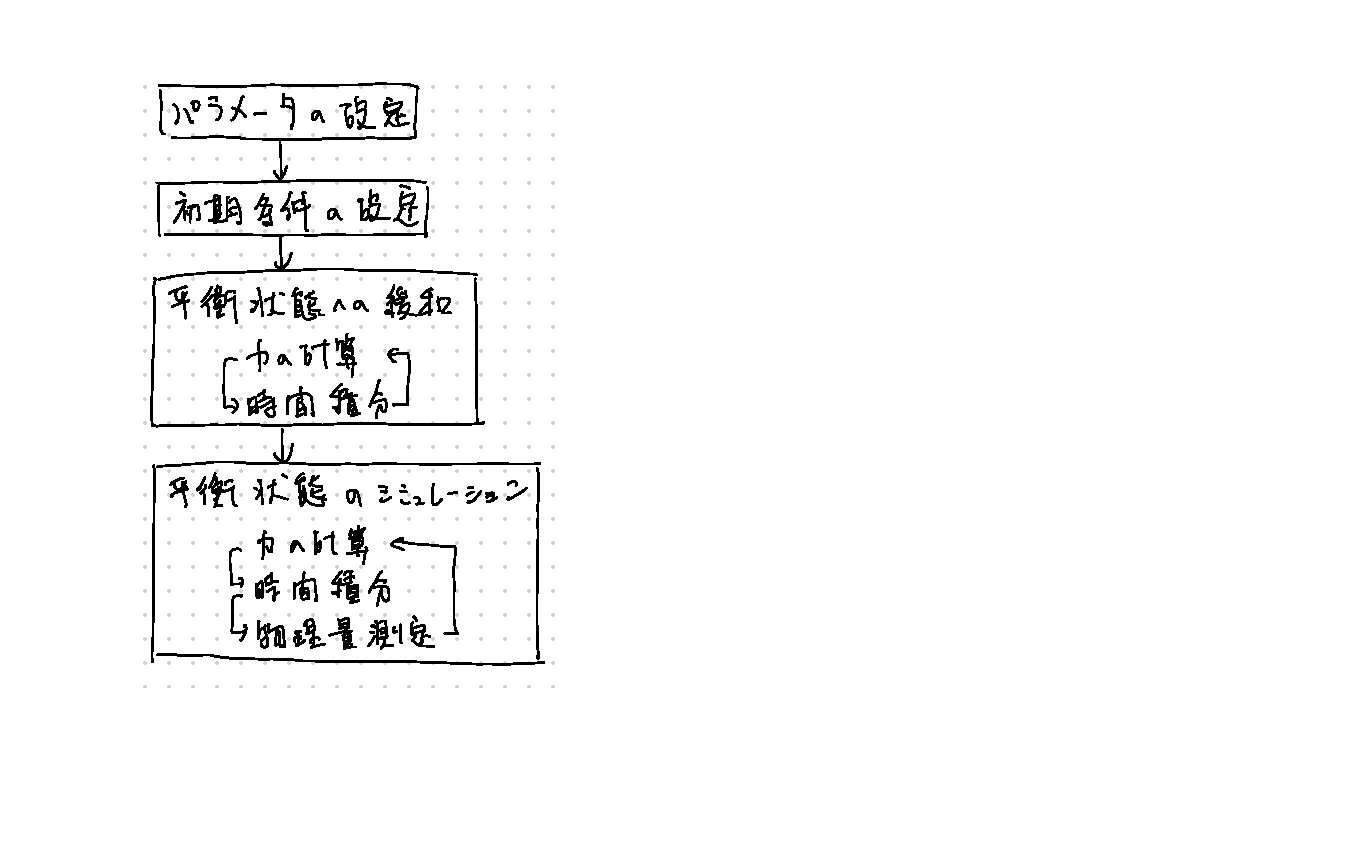
\includegraphics{image/md-flowchart.pdf}}
  \end{center}
\end{frame}

%%-*- coding:utf-8 -*-

\begin{frame}[t,fragile]{境界条件と力の計算}
  \begin{itemize}
    \setlength{\itemsep}{1em}
  \item 気体・液体・固体などの熱力学的極限を調べたい場合
    \begin{itemize}
    \item 端の効果を取り除くために周期境界条件を採用
    \item 周期的に同じパターンが続く
    \end{itemize}
  \item ポテンシャルの計算
    \begin{align*}
      U = \frac{1}{2} \sum_i \sum_{j \ne i} \sum_{n_x=-\infty}^{\infty} \sum_{n_y=-\infty}^{\infty} \sum_{n_z=-\infty}^{\infty} U[\mathbf{r}_i - \mathbf{r}_j + L(n_x,n_y,n_z)]
    \end{align*}
  \item 短距離力
    \begin{itemize}
    \item カットオフを入れる
    \item 最も近いイメージだけ考慮(minimum image convention)
    \end{itemize}
  \item 長距離力
    \begin{itemize}
    \item カットオフを入れると物理が変わる
    \item エバルト法、ツリー法、高速多重極展開
    \end{itemize}
  \end{itemize}
\end{frame}


% \section{常微分方程式の初期値問題(復習)}
\begin{frame}[t,fragile]{準備: 微分方程式の書き換え}
  \begin{itemize}
    %\setlength{\itemsep}{1em}
  \item 2階の常微分方程式の一般形
    \[
    \frac{d^2y}{dx^2} + p(x)\frac{dy}{dx} + q(x)y = r(x)
    \]
  \item $y_1 \equiv y$, $y_2 \equiv \frac{dy}{dx}$とおくと
    \[
    \left\{
    \begin{array}{ccl}
      \frac{dy_1}{dx} & = & y_2 \\
      \frac{dy_2}{dx} & = & r(x) - p(x) y_2 - q(x) y_1
    \end{array}
    \right.
    \]
  \item さらに$\bm{y}\equiv(y_1, y_2)$, $\bm{f}(x, \bm{y})\equiv \left(y_2, r(x)-p(x)y_2 - q(x)y_1\right)$
    \[
    \frac{d\bm{y}}{dx} = \bm{f}(x, \bm{y})
    \]
  \item $n$階常微分方程式 $\Rightarrow$ $n$次元の1階常微分方程式
  \end{itemize}
\end{frame}

\begin{frame}[t,fragile]{初期値問題の解法 (Euler法)}
  \begin{itemize}
    %\setlength{\itemsep}{1em}
  \item $h$を微小量として微分を差分で近似する(前進差分)
    \[
    \frac{dy}{dt} \approx \frac{y(t+h) - y(t)}{h} = f(t, y)
    \]
  \item $t=0$における$y(t)$の初期値を$y_0$、$t_n \equiv nh$、$y_n$を$y(t_n)$の近似値とおくと、
    \[
    y_{n+1}-y_n = h f( t_n, y_n)
    \]
  \item Euler法
    \begin{itemize}
    \item $y_0$からはじめて、$y_1,y_2,\cdots$を順次求めていく
    \end{itemize}
  \end{itemize}
\end{frame}

\begin{frame}[t,fragile]{高次のRunge-Kutta法}
  \begin{itemize}
    %\setlength{\itemsep}{1em}
  \item 3次Runge-Kutta法
    \[
    \begin{array}{rcl}
      k_1 & = & h f(t_n, y_n) \\
      k_2 & = & h f(t_n + \frac{2}{3}h, y_n + \frac{2}{3}k_1) \\
      k_3 & = & h f(t_n + \frac{2}{3}h, y_n + \frac{2}{3}k_2) \\
      y_{n+1} & = & y_n + \frac{1}{4}k_1 + \frac{3}{8}k_2
      + \frac{3}{8}k_3
    \end{array}
    \]
  \item 4次Runge-Kutta法
    \[
    \begin{array}{rcl}
      k_1 & = & h f(t_n, y_n) \\
      k_2 & = & h f(t_n + \frac{1}{2}h, y_n + \frac{1}{2}k_1) \\
      k_3 & = & h f(t_n + \frac{1}{2}h, y_n + \frac{1}{2}k_2) \\
      k_4 & = & h f(t_n + h, y_n + k_3) \\
      y_{n+1} & = & y_n + \frac{1}{6}k_1 + \frac{1}{3}k_2
      + \frac{1}{3}k_3 + \frac{1}{6}k_4
    \end{array}
    \]
  \item 4次までは次数と$f$の計算回数が等しい
  \end{itemize}
\end{frame}

\begin{frame}[t,fragile]{計算コストと精度}
  \begin{itemize}
    %\setlength{\itemsep}{1em}
  \item 実際の計算では$f(t,y)$の計算にほとんどのコストがかかる
  \item 計算回数と計算精度の関係
    \begin{center}
      \begin{tabular}[h]{c|cccc}
        & 1次(Euler法) & 2次(中点法) & 3次 & 4次 \\
        \hline
        計算精度 & $O(h)$ & $O(h^2)$ & $O(h^3)$ & $O(h^4)$ \\
        計算回数 & $N$ & $2N$ & $3N$ & $4N$
      \end{tabular}
    \end{center}
  \item 高次のRunge-Kuttaを使う方が効率的
  \item どれくらい小さな$h$が必要となるか、前もっては分からない
  \item 刻み幅を変えて($h,h/2,h/4,\dots$)計算してみることが大事
    \begin{itemize}
    \item 誤差の評価
    \item 公式の間違いの発見
    \end{itemize}
  \end{itemize}
\end{frame}


\section{シンプレクティック積分法}
\begin{frame}[t,fragile]{ハミルトン力学系}
  \begin{itemize}
    % \setlength{\itemsep}{1em}
  \item 時間をあらわに含まない場合のハミルトン方程式
    \[
    \frac{dq}{dt} = \frac{\partial H}{\partial p}, \ \frac{dp}{dt} = -\frac{\partial H}{\partial q}
    \]
    \begin{itemize}
    \item エネルギー保存則
      \[
      \frac{dH}{dt} = \frac{\partial H}{\partial q} \frac{dq}{dt} + \frac{\partial H}{\partial p} \frac{dp}{dt} = 0
      \]
    \item 位相空間の体積が保存(Liouvilleの定理)

      位相空間上の流れの場$\bm{v} = (\frac{dq}{dt},\frac{dp}{dt})$について
      \[
      \text{div} \bm{v} = \frac{\partial}{\partial q} \frac{dq}{dt} + \frac{\partial}{\partial p} \frac{dp}{dt} = 0
      \]
    \end{itemize}
  \item Euler法、Runge-Kutta法などはいずれの性質も満たさない
  \end{itemize}
\end{frame}

\begin{frame}[t,fragile]{シンプレクティック数値積分法(Symplectic Integrator)}
  \begin{itemize}
    %\setlength{\itemsep}{1em}
  \item 体積保存を満たす解法
  \item 例: 調和振動子$H=\frac{1}{2}(p^2+q^2)$の運動方程式
    \[
    \frac{dq}{dt} = p, \ \frac{dp}{dt} = -q
    \]
    の一方をEuler法で、他方を逆オイラー法で解く
    \begin{align*}
      q_{n+1} &= q_n + h p_n \\
      p_{n+1} &= p_n - h q_{n+1} = (1-h^2) p_n - h q_n \\
      \begin{pmatrix} q_{n+1} \\ p_{n+1} \end{pmatrix} &= \begin{pmatrix} 1 & h \\ -h & 1-h^2 \end{pmatrix} \begin{pmatrix} q_{n} \\ p_{n} \end{pmatrix}
    \end{align*}
  \end{itemize}
\end{frame}

\begin{frame}[t,fragile]{体積・エネルギーの保存}
  \begin{itemize}
    %\setlength{\itemsep}{1em}
  \item 体積保存
    \begin{align*}
      \det \begin{pmatrix} 1 & h \\ -h & 1-h^2 \end{pmatrix} = 1
    \end{align*}
  \item エネルギーの保存
    \begin{align*}
      \frac{1}{2}(p_{n+1}^2+q_{n+1}^2) + {\color{red}\frac{h}{2} p_{n+1} q_{n+1}} = \frac{1}{2}(p_{n}^2+q_{n}^2) + {\color{red}\frac{h}{2} p_{n} q_{n}}
    \end{align*}
  \item 位相空間の体積は厳密に保存
  \item エネルギーは$O(h)$の範囲で保存し続ける
  \end{itemize}
\end{frame}

\begin{frame}[t,fragile]{2次のシンプレクティック積分法}
  \begin{itemize}
    %\setlength{\itemsep}{1em}
  \item ハミルトニアンが$H(p,q) = T(p) + V(q)$の形で書けるとする
  \item リープ・フロッグ法
    \begin{align*}
      {\color{red} p(t+h/2)} &= p(t) - \frac{h}{2} \frac{\partial V(q)}{\partial q}|_{q=q(t)} \\
      {\color{blue} q(t+h)} &= q(t) + h {\color{red}p(t+h/2)} \\
      p(t+h) &= {\color{red}p(t+h/2}) - \frac{h}{2} \frac{\partial V(q)}{\partial q}|_{q=q(t+h)}
    \end{align*}
  \end{itemize}
\end{frame}


%\section{ベルレ法}
\begin{frame}[t,fragile]{ベルレ(Verlet)法}
  \begin{itemize}
    %\setlength{\itemsep}{1em}
  \item 微分方程式が$\ddot{q}(t) = f[t,q(t)]$の形で書かれる場合を考える
  \item $q(t)$のテイラー展開
    \[
    q(t \pm h) = q(t) \pm h \dot{q}(t) + \frac{h^2}{2} \ddot{q}(t) \pm \cdots
    \]
    から、$q(t + h)$と$q(t - h)$の表式を足し合わせて整理
    \[
    q(t+h) = 2q(t) - q(t-h)+h^2 f[t,q(t)] + O(h^4)
    \]
  \item 運動量の計算
    \[
    p(t) = \frac{q(t+h) - q(t-h)}{2h}
    \]
  \item 初期条件: $q(0)$と$p(0)$から$q(h)$を以下のように求める
    \[
    q(h) = q(0) + h p(0) + \frac{h^2}{2} f[0, q(0)]
    \]
  \end{itemize}
\end{frame}

\begin{frame}[t,fragile]{ベルレ法の変形}
  \begin{itemize}
    %\setlength{\itemsep}{1em}
  \item 半整数ステップにおける運動量
    \[
    p(t + h/2) = \frac{q(t+h)-q(t)}{h}
    \]
    を導入すると
    \begin{align*}
      \begin{split}
        p(t + h/2) &= p(t - h/2) + \frac{q(t+h)-2q(t)+q(t-h)}{h} \\
        &= p(t - h/2) + h f[t,q(t)]
      \end{split}
    \end{align*}
    一方
    \[
    q(t+h) = q(t) + hp(t+h/2)
    \]
  \item $\Rightarrow$ リープ・フロッグ法

    座標についてはベルレ法と数学的に等価だが、運動量の精度が高く、丸め誤差に強い
  \end{itemize}
\end{frame}

\begin{frame}[t,fragile]{速度ベルレ法(Velocity Verlet)}
  \begin{itemize}
    %\setlength{\itemsep}{1em}
  \item 運動量に対する中心差分
    \[
    p(t) = \frac{q(t+h)-q(t-h)}{2h}
    \]
    から
    \[
    q(t+h) = 2hp(t) + q(t-h)
    \]
    ベルレ法の式と和をとると
    \begin{align*}
      q(t + h) &= q(t) + hp(t) + h^2 f[t,q(t)] / 2 \\
      p(t + h) &= p(t) + h \Big( f[t+h,q(t+h)]  + f[t,q(t)] \Big) / 2
    \end{align*}
  \item $\Rightarrow$ 速度ベルレ法

    2次のシンプレクティック積分法、丸め誤差にも安定
  \end{itemize}
\end{frame}


%\section{シンプレクティック積分法の一般論}
\begin{frame}[t,fragile]{シンプレクティック法の一般論}
  \begin{itemize}
    %\setlength{\itemsep}{1em}
  \item $z=\begin{bmatrix} q \\ p \end{bmatrix}$と書き、$f(z)$に作用する演算子$\hat{D}(h)$をポアソン括弧を用いて定義($h=h(z)$はパラメータ)
    \[
    \hat{D}(h)f = \{ f, h \} = \frac{\partial f}{\partial q} \frac{\partial h}{\partial p} - \frac{\partial h}{\partial q} \frac{\partial f}{\partial p}
    \]
  \item ハミルトニアン$H=T(p)+V(q)$に対する正準方程式
    \[
    \dot{z} = \hat{D}(H) z
    \]
    に対する形式解
    \[
    z(t+h) = e^{h \hat{D}(H)} z(t)
    \]
  \item $e^{h \hat{D}(H)}$: 時間発展演算子 (正準変換)
  \end{itemize}
\end{frame}

\begin{frame}[t,fragile]{シンプレクティック法の一般論}
  \begin{itemize}
    %\setlength{\itemsep}{1em}
  \item $H=T(p)$の時
    \begin{align*}
      \hat{D}(T)z &= \frac{\partial z}{\partial q} \frac{\partial T}{\partial p} - \frac{\partial T}{\partial q} \frac{\partial z}{\partial p} = \begin{bmatrix} \frac{dT}{dp} \\ 0 \end{bmatrix} \\
      \hat{D}(T)^n z &= 0 \qquad n \ge 2 \\
      \therefore e^{h\hat{D}(T)} z &= [ 1+h\hat{D}(T) ] z = \begin{bmatrix} q + h \frac{dT}{dp} \\ p \end{bmatrix}
    \end{align*}
  \item $H=V(q)$の時も同様に
    \begin{align*}
      e^{h\hat{D}(V)} z &= [ 1+h\hat{D}(V) ] z = \begin{bmatrix} q \\ p - h \frac{dV}{dq} \end{bmatrix}
    \end{align*}
  \item $e^{h\hat{D}(T)}$, $e^{h\hat{D}(V)}$とも正準変換
  \item 一般的には、$e^{h\hat{D}(T+V)} z$は厳密には計算できない
  \end{itemize}
\end{frame}

\begin{frame}[t,fragile]{シンプレクティック法の一般論}
  \begin{itemize}
    %\setlength{\itemsep}{1em}
  \item $e^{h\hat{D}(T+V)}$を$e^{a_i h\hat{D}(T)}$, $e^{b_i h\hat{D}(V)}$の積で近似する
  \item 演算子(行列) $A,B$について
    \[
    e^{h (A+B)} = e^{hA} e^{hB} + O(h^2)
    \]
  \item 一次のシンプレクティック法
    \begin{align*}
      \hat{S}_1 &= e^{h\hat{D}(V)} e^{h\hat{D}(T)} \\
      q(t+h) &= q(t) + h \frac{dT(p(t))}{dp} \\
      p(t+h) &= p(t) - h \frac{dV(q({\color{red}t+h}))}{dq}
    \end{align*}
    $\Rightarrow$ オイラー法+逆オイラー法
  \end{itemize}
\end{frame}

\begin{frame}[t,fragile]{シンプレクティック法の一般論}
  \begin{itemize}
    %\setlength{\itemsep}{1em}
  \item 二次のシンプレクティック法
    \[
    e^{h (A+B)} = e^{\frac{h}{2}B} e^{hA} e^{\frac{h}{2}B} + O(h^3)
    \]
    から
    \begin{align*}
      \hat{S}_2 &= e^{\frac{h}{2}\hat{D}(T)} e^{h\hat{D}(V)} e^{\frac{h}{2}\hat{D}(T)}
    \end{align*}
    $\Rightarrow$ リープ・フロッグ法
  \item 四次のシンプレクティック法 (吉田の方法)
    \begin{align*}
      \hat{S}_4 &= e^{c_1h\hat{D}(T)} e^{d_1 h\hat{D}(V)} e^{c_2 h\hat{D}(T)} e^{d_2 h\hat{D}(V)} e^{c_3h\hat{D}(T)} e^{d_3 h\hat{D}(V)} e^{c_4h\hat{D}(T)} \\
      & c_1 = c_4 = \frac{1}{2(2-2^{1/3})}, \ c_2 = c_3 = \frac{1-2^{1/3}}{2(2-2^{1/3})}, \\
      & d_1 = d_3 = \frac{1}{2-2^{1/3}}, \ d_2 = \frac{2^{1/3}}{2-2^{1/3}}
    \end{align*}
  \end{itemize}
\end{frame}

\begin{frame}[t,fragile]{シンプレクティック積分法}
  \begin{itemize}
    \setlength{\itemsep}{1em}
  \item ハミルトン力学系の満たすべき特性(位相空間の体積保存)を満たす
  \item 一般的には陰解法
  \item ハミルトニアンが$H(p,q) = T(p) + V(q)$の形で書ける場合は陽的なシンプレクティック積分法が存在する
  \item エネルギーは近似的に保存する
  \item $n$次のシンプレクティック積分法では、エネルギーは$O(h^n)$の範囲で振動(発散しない)
  \end{itemize}
\end{frame}


%\section{分子動力学法}

%%-*- coding:utf-8 -*-

\begin{frame}[t,fragile]{分子動力学法}
  \begin{itemize}
    \setlength{\itemsep}{1em}
  \item 適当な初期条件から、運動方程式に従って位置と運動量を時間発展させる
    \begin{itemize}
    \item Euler法、Runge-Kutta法、リープ・フロッグ法、速度ベルレ法など
    \item $6N$次元の連立微分方程式
    \end{itemize}
  \item 時間発展に関する物理量の時間平均から平均を評価
    \begin{align*}
      \langle A(p,x) \rangle &= \frac{1}{Z(E)} \int A(p,x) \, \delta(H(p,x)-E) \, dp \, dx \\
      &\simeq \frac{1}{t_{\rm max}} \int_0^{t_{\rm max}} A(p(t),x(t)) \, dt
    \end{align*}
    \begin{itemize}
    \item 運動方程式では全エネルギーが保存する→ミクロカノニカル分布
    \end{itemize}
  \item 平衡状態における平均値だけでなく、熱や電荷の輸送などの動的現象、非平衡状態からの緩和現象などもシミュレーションできる
  \end{itemize}
\end{frame}

%%-*- coding:utf-8 -*-

\begin{frame}[t,fragile]{フローチャート}
  \begin{center}
    \resizebox{0.45\textwidth}{!}{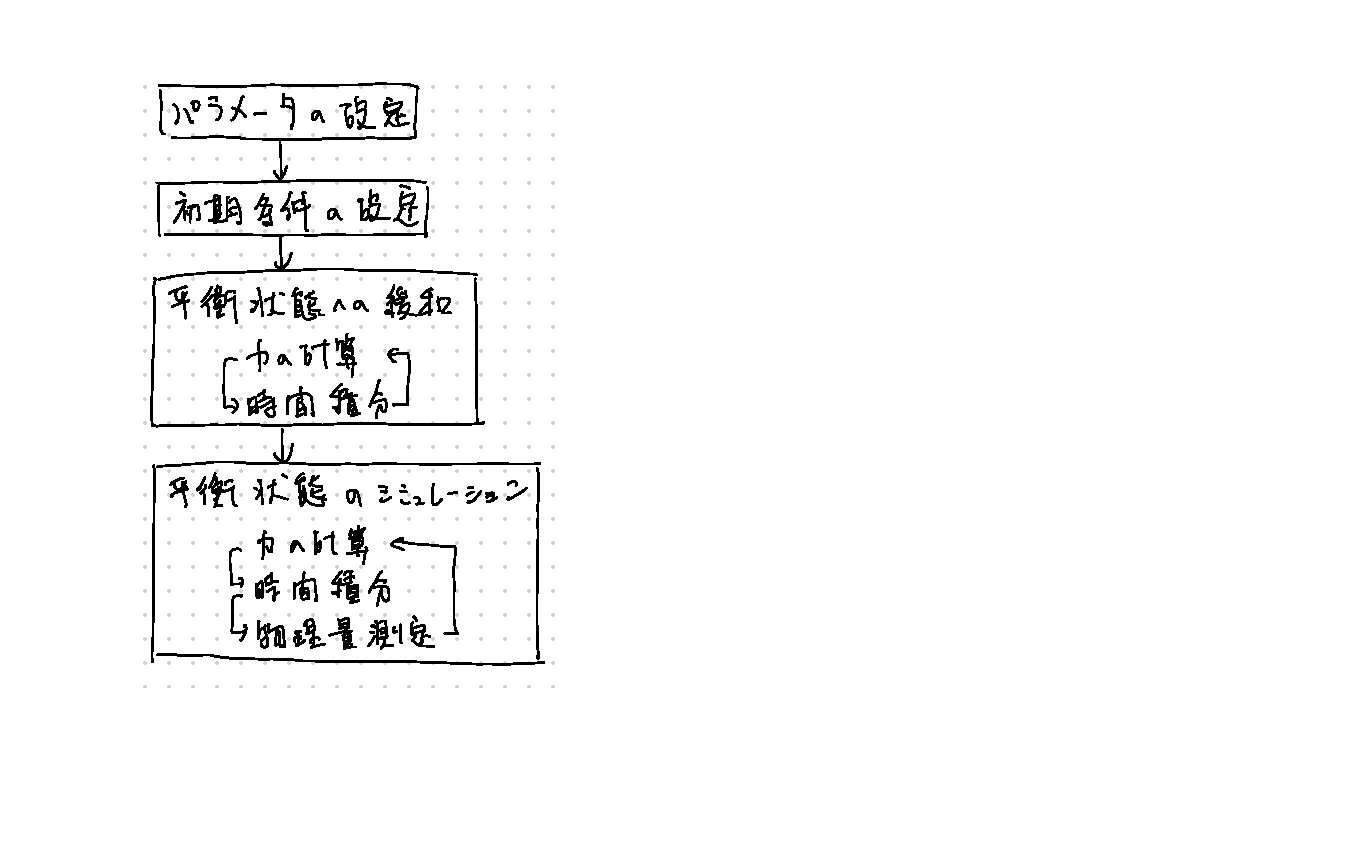
\includegraphics{image/md-flowchart.pdf}}
  \end{center}
\end{frame}


\section{長距離ポテンシャルの計算}

%-*- coding:utf-8 -*-

\begin{frame}[t,fragile]{境界条件と力の計算}
  \begin{itemize}
    \setlength{\itemsep}{1em}
  \item 気体・液体・固体などの熱力学的極限を調べたい場合
    \begin{itemize}
    \item 端の効果を取り除くために周期境界条件を採用
    \item 周期的に同じパターンが続く
    \end{itemize}
  \item ポテンシャルの計算
    \begin{align*}
      U = \frac{1}{2} \sum_i \sum_{j \ne i} \sum_{n_x=-\infty}^{\infty} \sum_{n_y=-\infty}^{\infty} \sum_{n_z=-\infty}^{\infty} U[\mathbf{r}_i - \mathbf{r}_j + L(n_x,n_y,n_z)]
    \end{align*}
  \item 短距離力
    \begin{itemize}
    \item カットオフを入れる
    \item 最も近いイメージだけ考慮(minimum image convention)
    \end{itemize}
  \item 長距離力
    \begin{itemize}
    \item カットオフを入れると物理が変わる
    \item エバルト法、ツリー法、高速多重極展開
    \end{itemize}
  \end{itemize}
\end{frame}

%-*- coding:utf-8 -*-

\begin{frame}[t,fragile]{エバルト法}
  \begin{itemize}
    %\setlength{\itemsep}{1em}
  \item 周期的なクーロンポテンシャル(粒子数$N$)
    \[
    U = \frac{1}{2} \sum_{i,j} \sum_{\mathbf{n}} \frac{q_i q_j}{r} \qquad r = |\mathbf{r}| = |\mathbf{r}_i - \mathbf{r}_j + L \mathbf{n}|
    \]
  \item 無限個のミラーイメージに関する和をいかに計算するか
    \begin{itemize}
    \item 誤差関数(erf)と相補誤差関数(erfc)を用いて、ポテンシャルを2つの部分に分ける($\alpha$はある定数)
      \[
      U = \frac{1}{2} \sum_{i,j} \sum_{\mathbf{n}} \frac{q_i q_j \, \mathrm{erfc}(\alpha r)}{r} + \frac{1}{2} \sum_{i,j} \sum_{\mathbf{n}} \frac{q_i q_j \, \mathrm{erf}(\alpha r)}{r}
      \]
    \item 第1項目は$r$が大きくなると急速に小さくなる
    \end{itemize}
  \end{itemize}
\end{frame}

%-*- coding:utf-8 -*-

\begin{frame}[t,fragile]{エバルト法}
  \begin{itemize}
    %\setlength{\itemsep}{1em}
  \item 第2項目(長距離項)の計算
    \begin{itemize}
    \item 変数変換($s=t/r$)
      \[
      \begin{split}
        U_2 &= \frac{1}{2} \sum_{i,j} \sum_{\mathbf{n}} \frac{q_i q_j}{r} \frac{2}{\sqrt{\pi}} \int_0^{\alpha r} \exp(-t^2) \, dt \\
        &= \frac{1}{2} \sum_{i,j} q_i q_j  \frac{2}{\sqrt{\pi}} \int_0^{\alpha} \sum_{\mathbf{n}} \exp(-r^2 s^2) \, ds
        \end{split}
      \]
    \item 被積分関数は$\mathbf{r}_i$に関して周期$L$の周期関数$\rightarrow$フーリエ変換を導入
      \[
      U_2 = \frac{2\pi}{L^3} \sum_{\mathbf{h} \ne \mathbf{0}} \frac{e^{-|\mathbf{h}|^2/4\alpha^2}}{|\mathbf{h}|^2} \Big| \sum_i q_i e^{i\mathbf{h} \cdot \mathbf{r}_i} \Big|^2 \qquad \mathbf{h} = \frac{2\pi}{L}(h_x, h_y, h_z)
      \]
    \item $|\mathbf{h}|$が大きくなると急速に小さくなる
    \item $\mathbf{h} = \mathbf{0}$の項は電気的中性条件から消える
    \end{itemize}
  \end{itemize}
\end{frame}


%-*- coding:utf-8 -*-

\begin{frame}[t,fragile]{ツリー法}
  \begin{itemize}
    %\setlength{\itemsep}{1em}
  \item 遠くのものをまとめて扱う
  \item 空間をメッシュで8等分(2次元の場合は4等分)していく
    \begin{center}
      \resizebox{!}{.4\textheight}{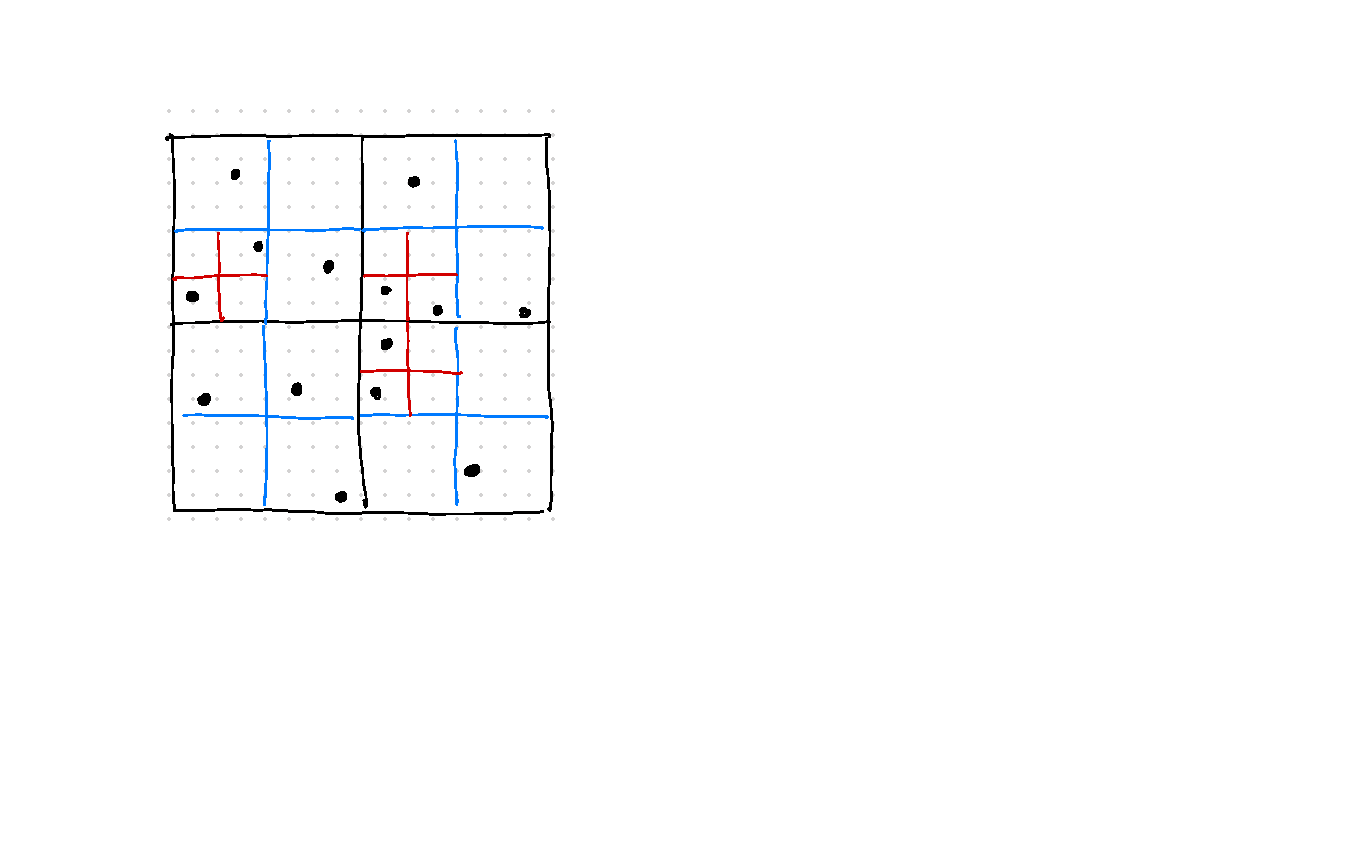
\includegraphics{image/tree-1.pdf}}
      \resizebox{!}{.4\textheight}{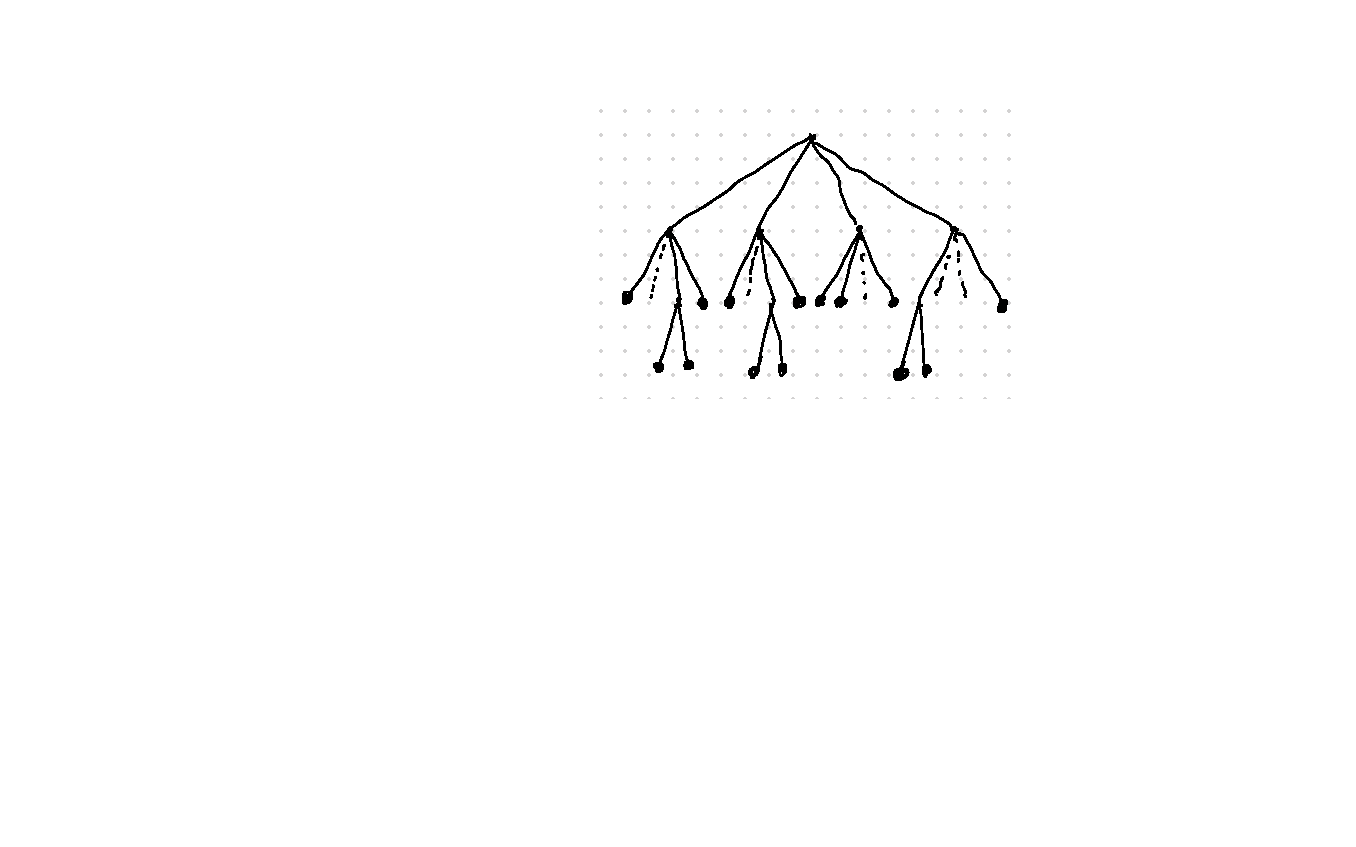
\includegraphics{image/tree-2.pdf}}
    \end{center}
    \begin{itemize}
    \item それぞれのメッシュに粒子が1個あるいは0個となるまで
    \item 全体が8分木(2次元の場合は4分木)で表現される
    \item ツリー構造の下から順番に重心と総質量を計算しておく
    \end{itemize}
  \end{itemize}
\end{frame}


%-*- coding:utf-8 -*-

\begin{frame}[t,fragile]{ツリー法}
  \begin{itemize}
    %\setlength{\itemsep}{1em}
  \item ある粒子から見て
    \begin{itemize}
    \item 見込み角があるしきい値よりも小さい場合は、その重心を使って計算
    \item そうでない場合にはまじめに計算
    \end{itemize}
  \item 計算量 $O(N \log N)$
  \item 近似精度を上げるには
    \begin{itemize}
    \item 見込み角のしきい値を小さくする→計算量が急速に増える
    \item 重心だけでなく多重極展開も使う

      原点中心半径$a$の球の中の粒子の作るポテンシャルの多重極展開係数
      \[
      \alpha_\ell^m = \sum_{i=1}^{N} m_i \Big( \frac{r_i}{a} \Big)^\ell Y_\ell^{-m}(\theta_i, \phi_i)
      \]
      $Y_\ell^m(\theta,\phi)$: $\ell$次の球面調和関数

      位置$(r,\theta,\phi)$におけるポテンシャル($r>a$)
      \[
      \Phi(r,\theta,\phi) \approx \sum_\ell \sum_{m=-\ell}^{\ell} \alpha_\ell^m \frac{a^\ell}{r^{\ell+1}} Y_\ell^m(\theta,\phi)
      \]
      
    \end{itemize}
  \end{itemize}
\end{frame}



\section{ビリアル定理}

%-*- coding:utf-8 -*-

\begin{frame}[t,fragile]{ビリアル定理}
  \begin{itemize}
    %\setlength{\itemsep}{1em}
  \item ビリアル定理
    \[
    \langle T \rangle = -\frac{1}{2} \sum_i^N \langle \mathbf{f}_i \cdot \mathbf{r}_i \rangle
    \]
    $T$: 運動エネルギー、$\mathbf{f}_i$: 粒子$i$に働く力、$\mathbf{r}_i$: 粒子$i$の位置
  \item ビリアル
    \[
    G = \sum_i^N \mathbf{p}_i \cdot \mathbf{r}_i
    \]
    \begin{itemize}
    \item $G$の時間微分
      \[
      \frac{dG}{dt} = \sum_i \mathbf{p}_i \cdot \frac{d\mathbf{r}_i}{dt} + \sum_i \frac{d\mathbf{p}_i}{dt} \cdot \mathbf{r}_i = 2 T + \sum_i \mathbf{f}_i \cdot \mathbf{r}_i
      \]
    \item 長時間平均をとると左辺は0 $\Rightarrow$ ビリアル定理
    \end{itemize}
  \end{itemize}
\end{frame}

%-*- coding:utf-8 -*-

\begin{frame}[t,fragile]{ビリアル定理}
  \begin{itemize}
    %\setlength{\itemsep}{1em}
  \item ベキ的な相互作用の場合: $U = \sum_{i<j} a_{ij} | \mathbf{r}_i - \mathbf{r}_j |^{n+1}$
    \[
    \mathbf{f}_i = -\nabla_i U = - \sum_{j \ne i} a_{ij} (n+1) (\mathbf{r}_i - \mathbf{r}_j) | \mathbf{r}_i - \mathbf{r}_j |^{n-1} \equiv \sum_{j \ne i} \mathbf{f}_{ij}
    \]
    \begin{align*}
      -\frac{1}{2} \sum_i \mathbf{f}_i \cdot \mathbf{r}_i &= -\frac{1}{2} \sum_i \sum_{j \ne i} \mathbf{f}_{ij} \cdot \mathbf{r}_i = -\frac{1}{2} \sum_{i < j} (\mathbf{f}_{ij} \cdot \mathbf{r}_i + \mathbf{f}_{ji} \cdot \mathbf{r}_j) \\
      &= -\frac{1}{2} \sum_{i < j} \mathbf{f}_{ij} \cdot (\mathbf{r}_i - \mathbf{r}_j) = \frac{1}{2} (n+1) U
    \end{align*}
    $\Rightarrow$ $\displaystyle \langle T \rangle = \frac{n+1}{2} \langle U \rangle$
  \item 特に重力、静電気力の場合($n=-2$)
    \[
     \langle T \rangle = -\frac{1}{2} \langle U \rangle \qquad \text{ビリアル比: $\displaystyle r_{\rm v} \equiv \frac{\langle T \rangle}{| \langle U \rangle |} = \frac{1}{2}$}
    \]
  \end{itemize}
\end{frame}

%-*- coding:utf-8 -*-

\begin{frame}[t,fragile]{圧力・温度の計算}
  \begin{itemize}
    %\setlength{\itemsep}{1em}
  \item 壁から受ける力を考えると
    \begin{align*}
    \mathbf{f}_i &= \mathbf{f}_i^\text{int} + \mathbf{f}_i^\text{ext} = -\nabla_i U + \mathbf{f}_i^\text{ext} \\
      \mathbf{f}_i^\text{ext} &= - \int_{\partial V} (P \mathbf{n}) \cdot \mathbf{r} \, dS = - P \int \nabla \cdot \mathbf{r} \, dV = -3PV
    \end{align*}
  \item ビリアル定理と組み合わせて
    \[
    PV = \frac{2}{3} \langle T \rangle -\frac{1}{3} \langle \sum_i \nabla_i U \cdot \mathbf{r}_i \rangle
    \]
  \item 温度の計算: エネルギー等分配則より
    \[
    \langle T \rangle = \frac{3}{2} k_B T N
    \]
    %\begin{itemize}
    %\item
    (全運動量を0に固定している場合は$\langle T \rangle = \frac{3}{2} k_B T (N-1)$)
    %\end{itemize}
  \end{itemize}
\end{frame}


\section{温度の制御}

%-*- coding:utf-8 -*-

\begin{frame}[t,fragile]{温度の制御}
  \begin{itemize}
    %\setlength{\itemsep}{1em}
  \item カノニカル分布を実現するには?
    \begin{itemize}
    \item 巨大な環境(熱浴)を付ける必要がある?
    \item シミュレーションで巨大な環境を用意するのは非現実的
    \end{itemize}
  \item 速度スケーリング(Velocity Scaling)法
    \begin{itemize}
    \item 平均の運動エネルギーが対応する温度に一致するように毎回速度(運動量)をスケールしなおす
      \begin{align*}
        p_i \Rightarrow &p'_i = \sqrt{ \frac{3mNk_BT}{\sum_i p_i^2} } p_i \\
        & \sum_i \frac{p_i^{'2}}{2m} = \frac{3mNk_BT}{\sum_i p_i^2} \sum_i \frac{p_i^2}{2m} = \frac{3}{2} N k_B T
      \end{align*}
    \item 位置エネルギーも運動エネルギーに引きずられてカノニカル分布に収束? $\Rightarrow$ 理論的根拠なし
    \end{itemize}
  \end{itemize}
\end{frame}

%-*- coding:utf-8 -*-

\begin{frame}[t,fragile]{温度の制御}
  \begin{itemize}
    %\setlength{\itemsep}{1em}
  \item ランジュバン(Langevin)法
    \begin{itemize}
    \item 乱数を使う方法
    \item 摩擦項と揺動項(ランダム力)を付け加える
      \begin{align*}
        \frac{dp_i}{dt} = - \frac{\partial H}{\partial q_i} - \gamma_i p_i + R_i(t)
      \end{align*}
    \item $\gamma_i$: 摩擦係数
    \item $R_i(T)$: 平均零の白色ノイズ
      \begin{align*}
        \langle R_i(t) R_i(t') \rangle = 2 m \gamma_i k_B T \delta(t-t')
      \end{align*}
    \item 摩擦項と揺動項がつりあうところで、温度$T$のカノニカル分布が実現する
    \end{itemize}
  \end{itemize}
\end{frame}

%-*- coding:utf-8 -*-

\begin{frame}[t,fragile]{Nose-Hoover熱浴}
  \begin{itemize}
    %\setlength{\itemsep}{1em}
  \item Nose (能勢)-Hoover法
    \begin{itemize}
    \item 熱浴をたった1つの自由度($s$)だけで実現する!
    \item 現実系のハミルトニアン
      \begin{align*}
        H(\mathbf{p},\mathbf{x}) &= \sum_i \frac{p_i^2}{2m} + U(\mathbf{x})
      \end{align*}
    \item 仮想系のハミルトニアン (温度$T$をパラメータとして含む)
      \begin{align*}
        H'(\mathbf{p}',\mathbf{x}',{\color{red}p_s},{\color{red}s}) &= \sum_i \frac{{p'_i}^2}{2m{\color{red}s^2}} + U(\mathbf{x}') + {\color{red}\frac{p_s^2}{2Q} + g k_B T\log s}
      \end{align*}
      $s$: 熱浴の自由度、$p_s$: $s$に共役な運動量、$Q$: 熱浴の「質量」、$g$: 系の自由度($3N+1$または$3N$)
    \end{itemize}
  \end{itemize}
\end{frame}


%-*- coding:utf-8 -*-

\begin{frame}[t,fragile]{Nose-Hoover熱浴}
  \begin{itemize}
  \item 仮想系の運動方程式
    \begin{align*}
      \frac{dx_i'}{dt'} &= \frac{\partial H'}{\partial p_i'} = \frac{p_i'}{ms^2} \\
      \frac{dp_i'}{dt'} &= -\frac{\partial H'}{\partial x_i'} = -\frac{\partial U}{\partial x_i'} \\
      \frac{ds}{dt'} &= \frac{\partial H'}{\partial p_s} = \frac{p_s}{Q} \\
      \frac{dp_s}{dt'} &= -\frac{\partial H'}{\partial s} = \sum_i \frac{{p'_i}^2}{ms^3} - \frac{g k_B T}{s}
    \end{align*}
  \item 現実系と仮想系との間に以下の関係を仮定する

    $x_i=x_i'$、$p_i=p_i'/{\color{red}s}$、$t=\int^t s^{-1} dt'$、$dt=dt'/{\color{red}s}$
  \end{itemize}
\end{frame}

%-*- coding:utf-8 -*-

\begin{frame}[t,fragile]{Nose-Hoover熱浴}
  \begin{itemize}
    %\setlength{\itemsep}{1em}
  \item 現実系の変数による書き換え
    \begin{align*}
      \frac{dx_i}{dt} &= \frac{\partial H}{\partial p_i} \\
      \frac{dp_i}{dt} &= -\frac{\partial U}{\partial x_i} -\frac{p_s}{Q} p_i \\
      \frac{dp_s}{dt} &= 2 \big[ \sum_i \frac{{p_i}^2}{2m} - \frac{g k_B T}{2} \big]
    \end{align*}
  \item あるいは、$x_s = \log s$を導入すると、最後の2つの式は
    \begin{align*}
      % \frac{dx_i}{dt} &= \frac{\partial H}{\partial p_i} \\
      \frac{dp_i}{dt} &= -\frac{\partial U}{\partial x_i} -\frac{dx_s}{dt} p_i \\
      \frac{d^2x_s}{dt^2} &= \frac{2}{Q} \big[ \sum_i \frac{{p_i}^2}{2m} - \frac{g k_B T}{2} \big]
    \end{align*}
  \end{itemize}
\end{frame}

%-*- coding:utf-8 -*-

\begin{frame}[t,fragile]{カノニカル分布の実現}
  \begin{itemize}
    %\setlength{\itemsep}{1em}
  \item $H'(\mathbf{p}',\mathbf{x}',p_s,s)$による仮想時間発展によりエネルギー$E'$のミクロカノニカルアンサンブルが実現しているとする

    $\Leftrightarrow$ 仮想時間$t'$でサンプルすると$2(3N+1)$次元の位相空間上で$H'=E$の曲面上に均等に分布(エルゴード性)
    
    $\Leftrightarrow$ 分布関数: $\delta [ H'(\mathbf{p}',\mathbf{x}',p_s,s) - E']$
    
    $\Rightarrow$ 現実系の変数$(p,q)$に関する周辺分布を考える
  \item 仮想系のミクロカノニカル分配関数
    \begin{align*}
      Z'&=\int d\mathbf{p}' d\mathbf{x}' dp_s ds \, \delta [ H'(\mathbf{p}',\mathbf{x}',p_s,s) - E'] \\
      &=\int d\mathbf{{\color{red}p}} d\mathbf{{\color{red}x}} dp_s ds \, {\color{red}s^{3N}} \delta [ {\color{red}H(\mathbf{p},\mathbf{x})} + \frac{p_s^2}{2Q} + g k_B T \log s - E']
    \end{align*}
  \end{itemize}
\end{frame}

%-*- coding:utf-8 -*-

\begin{frame}[t,fragile]{カノニカル分布の実現}
  \begin{itemize}
    %\setlength{\itemsep}{1em}
  \item $s$について積分(*)
    \begin{align*}
      \int ds \, s^{3N} \delta[f(s)] = s_0^{3N} / | f'(s_0) | = s_0^{3N+1} / g k_B T
    \end{align*}
    $f(s) \equiv H(\mathbf{p},\mathbf{x}) + \frac{p_s^2}{2Q} + g k_B T \log s - E'$、$s_0$は$f(s)=0$の解
    \begin{align*}
      s_0 = \exp \Big[ -\frac{1}{gk_BT} \Big( H(p,x) + \frac{p_s^2}{2Q} - E' \Big) \Big]
    \end{align*}
  \item さらに$p_s$についてガウス積分を行い、$g=3N+1$とすると
    \begin{align*}
      Z' = \frac{1}{3N+1} \sqrt{\frac{2Q\pi}{k_BT}} e^{E'/k_BT} \int d\mathbf{p}d\mathbf{x} \, {\color{red}\exp [- H(p,x)/k_BT ]}
    \end{align*}
  \end{itemize}
\end{frame}

%%-*- coding:utf-8 -*-

\begin{frame}[t,fragile]{補足(*)}
  \begin{itemize}
    %\setlength{\itemsep}{1em}
  \item $f(s)=0$の解を$s_0$とすると、$\displaystyle \delta [f(s)] = \frac{\delta(s-s_0)}{|f'(s_0)|}$が成り立つ

    証明: $u=f(s)$とおくと、$du = f'(s)ds$から
    \begin{align*}
      \int h(s) {\color{red}\delta [f(s)]} \, ds= \int h(f^{-1}(u)) \delta(u) \frac{du}{|f'(f^{-1}(u))|}
    \end{align*}
    $f^{-1}(0)=s_0$なので
    \begin{align*}
      = \frac{h(s_0)}{|f'(s_0)|} = \int h(s) {\color{red}\frac{\delta(s-s_0)}{|f'(s_0)|}} ds
    \end{align*}
  \end{itemize}
\end{frame}

%-*- coding:utf-8 -*-

\begin{frame}[t,fragile]{実時間発展の場合}
  \begin{itemize}
    %\setlength{\itemsep}{1em}
  \item 実時間に直した方程式の時間発展を計算した場合、物理量$A(\mathbf{p},\mathbf{x})$の実時間平均は
    \begin{align*}
      \langle A \rangle_t &= \lim_{\tau\rightarrow\infty} \frac{1}{\tau} \int_0^\tau dt \, A(\mathbf{p}(t),\mathbf{x}(t)) \\
      &= \lim_{\tau\rightarrow\infty} \frac{\tau'}{\tau} \frac{1}{\tau'} \int_0^{\tau'} dt' \, A(\mathbf{p}'(t')/s(t'),\mathbf{x}'(t')) / s(t')
    \end{align*}
  \item $\tau = \int_0^{\tau} dt = \int_0^{\tau'} dt'/s(t')$なので
    \begin{align*}
      \langle A \rangle_t &= \frac{\lim_{\tau'\rightarrow\infty} \frac{1}{\tau'} \int_0^{\tau'} dt' \, A(\mathbf{p}'(t')/s(t'),\mathbf{x}'(t')) / s(t')}{\lim_{\tau'\rightarrow\infty} \frac{1}{\tau'} \int_0^{\tau'} dt' \, 1/ s(t')} \\
      &= \langle A(\mathbf{p},\mathbf{x}) / s \rangle_{t'} / \langle 1 / s \rangle_{t'}
    \end{align*}
  \end{itemize}
\end{frame}

%-*- coding:utf-8 -*-

\begin{frame}[t,fragile]{実時間発展の場合}
  \begin{itemize}
    %\setlength{\itemsep}{1em}
  \item 分子・分母の$t'$に関する期待値を計算すると、$s_0$が1つキャンセルするので
    \begin{align*}
      \langle A \rangle_t &= \frac{\int d\mathbf{p} d\mathbf{x} \, A(\mathbf{p},\mathbf{x}) \exp [ -\frac{3N}{gk_BT} H(\mathbf{p}, \mathbf{x})]}{\int d\mathbf{p} d\mathbf{x} \, \exp [ -\frac{3N}{gk_BT} H(\mathbf{p}, \mathbf{x})]}
    \end{align*}
    \item {\color{red}$g=3N$}とすると、実時間発展の長時間平均とカノニカル分布における位相平均が一致
  \end{itemize}
\end{frame}

%-*- coding:utf-8 -*-

\begin{frame}[t,fragile]{温度の制御}
  \begin{itemize}
    %\setlength{\itemsep}{1em}
  \item Nose-Hoover熱浴
    \begin{itemize}
    \item 運動方程式(実時間発展の場合)
      \begin{align*}
        \frac{dx_i}{dt} &= \frac{\partial H}{\partial p_i} \\
        \frac{dp_i}{dt} &= -\frac{\partial U}{\partial x_i} -\frac{p_s}{Q} p_i \\
        \frac{dp_s}{dt} &= 2 \big[ \sum_i \frac{{p_i}^2}{2m} - \frac{g k_B T}{2} \big]
      \end{align*}
    \item 「摩擦係数」$p_s$にネガティブフィードバックがかかる
    \item $g=3N$ととれば、$(p,x)$の周辺分布はカノニカル分布になる
    \end{itemize}
  \item 調和振動子系など簡単な系では保存量が生じてエルゴード性が破れる場合も $\Rightarrow$ 自由度$s$の温度を制御するもう一つの自由度$r$を追加(Nose-Hoover Chain法) 
  \item 温度圧力一定(NPTアンサンブル)も体積を表すもう1つの自由度を追加することで実現可
  \end{itemize}
\end{frame}


\end{document}
